\documentclass[12pt,a4paper]{article}

\usepackage[a4paper,margin=1in]{geometry}
\usepackage{graphicx}
\usepackage{booktabs}
\usepackage{amsmath,amssymb}
\usepackage{float}
\usepackage{hyperref}
\usepackage{xcolor}
\usepackage{listings}
\usepackage{enumitem}
\usepackage{fancyhdr}
\usepackage{longtable}

\hypersetup{colorlinks=true,linkcolor=blue,urlcolor=blue}

\pagestyle{fancy}
\fancyhf{}
\lhead{ICS1512}
\rhead{Machine Learning Algorithms Laboratory}
\cfoot{\thepage}

\lstset{
language=Python,
basicstyle=\ttfamily\small,
numbers=left,
frame=single,
breaklines=true,
showstringspaces=false
}

\begin{document}

\begin{tabular}{|p{4cm}|p{11cm}|}
\hline
Experiment No. & 2 \\ \hline
Experiment Title & Email Spam/Ham Classification using Na\"ive Bayes and KNN
\footnote{\textbf{GitHub Repository: }\url{https://github.com/username/repository}}\\ \hline
Student Name & \\ \hline
Register Number & \\ \hline
Faculty & Dr. Poreddy Ajay Kumar Reddy \\ \hline
Submission Date & \\ \hline
\end{tabular}

\section{Objective}
\begin{itemize}
\item Build spam classifiers using Na\"ive Bayes and K-Nearest Neighbors (KNN).
\item Compare Gaussian, Multinomial, and Bernoulli Na\"ive Bayes variants.
\item Study the effect of varying the number of neighbors $k$ in KNN.
\item Compare the KDTree and BallTree nearest-neighbor search algorithms.
\item Optimize KNN hyperparameters using GridSearchCV and RandomizedSearchCV.
\item Evaluate the computational (training/prediction) time of each algorithm.
\item Evaluate model performance using 5-fold Cross Validation.
\end{itemize}

\section{Problem Statement}
Given a dataset of emails represented by 57 numeric features describing word/character
frequencies and capital-letter run-length statistics, the task is to classify each email
as \textbf{spam} (1) or \textbf{ham/not-spam} (0).
\begin{itemize}
\item \textbf{Input:} 57 continuous numeric features per email (word frequencies,
character frequencies, and capital-run-length statistics).
\item \textbf{Process:} Load and clean the data, perform EDA, scale features
appropriately for each classifier, train and compare Na\"ive Bayes variants (Gaussian,
Multinomial, Bernoulli) and KNN, tune KNN hyperparameters via GridSearchCV and
RandomizedSearchCV, compare KDTree vs.\ BallTree, and evaluate all models using 5-fold
cross validation.
\item \textbf{Output:} A binary class label (spam / ham) for each email, along with a
comparative analysis of classifier accuracy, robustness, and computational cost.
\end{itemize}

\section*{Theory}
Na\"ive Bayes is a probabilistic classifier based on Bayes' theorem, which assumes
conditional independence between features given the class:
\begin{equation}
P(C \mid X) = \frac{P(X \mid C)\,P(C)}{P(X)}
\end{equation}
where $C$ is the class label (spam/ham) and $X$ is the feature vector of an email.
Three variants were compared: \textbf{Gaussian NB} (assumes features follow a normal
distribution within each class), \textbf{Multinomial NB} (models discrete counts /
frequencies, suited to word-frequency style features), and \textbf{Bernoulli NB}
(models binary presence/absence of features).

KNN is a lazy, instance-based learning algorithm that classifies a query sample based on
the majority class among its $k$ nearest neighbors in feature space, using a distance
metric such as Euclidean or Manhattan distance. Since KNN performs no explicit training
phase, all computation is deferred to prediction time, when distances to (a subset of)
the training points must be computed. KDTree and BallTree are spatial indexing
structures that accelerate this nearest-neighbor search compared to a brute-force scan.

\section{Dataset Description}
\begin{longtable}{|p{6cm}|p{8cm}|}
\hline
Dataset Name & Spambase Dataset \\ \hline
Dataset Source & UCI Machine Learning Repository / Kaggle (\url{https://www.kaggle.com/datasets/somesh24/spambase}) \\ \hline
Number of Samples & 4601 \\ \hline
Number of Features & 57 numeric features (word frequency, character frequency, capital-run-length statistics) \\ \hline
Number of Classes & 2 (Spam = 1: 1813 samples; Ham = 0: 2788 samples) \\ \hline
Missing Values & 0 (none found) \\ \hline
Train-Test Split & 75\% train (3450 samples) / 25\% test (1151 samples), stratified, \texttt{random\_state=42} \\ \hline
\end{longtable}

\textit{Note: the notebook was executed using the header-less UCI distribution of the
dataset (\texttt{spambase.data}, 57 features + 1 label column), so features are
referenced by their positional names \texttt{f0}--\texttt{f56} throughout this report,
exactly as produced by the executed pipeline.}

\section{Exploratory Data Analysis}
EDA was performed on the raw 57-feature email dataset prior to any scaling.

\begin{itemize}
\item \textbf{Dataset overview:} 4601 emails $\times$ 57 numeric features + 1 binary
target (\texttt{spam}).
\item \textbf{Missing value analysis:} No missing values were found in any column; no
imputation was required.
\item \textbf{Class distribution:} 2788 ham emails (60.6\%) and 1813 spam emails
(39.4\%) -- a moderate class imbalance.
\item \textbf{Correlation matrix:} Computed for the top 15 features most correlated
with the target, most inter-feature correlations are weak-to-moderate, with feature
\texttt{f24} showing a notable negative correlation with several other top features.
\item \textbf{Feature distribution:} The top 4 most target-correlated features
(\texttt{f20}, \texttt{f22}, \texttt{f6}, \texttt{f52}) are strongly right-skewed,
with most values concentrated near zero and a long tail of larger values, more
pronounced for spam emails.
\end{itemize}

\begin{figure}[H]
\centering
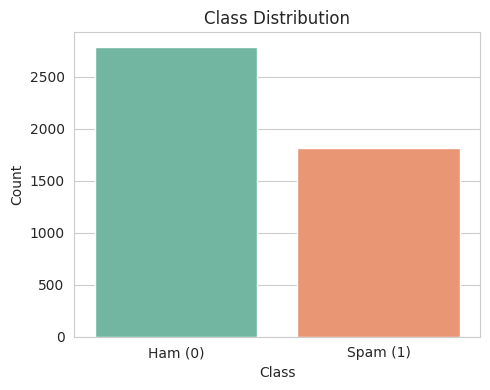
\includegraphics[width=0.6\linewidth]{images/fig01_class_distribution.png}
\caption{Class distribution of the Spambase dataset (Ham = 0, Spam = 1).}
\label{fig:classdist}
\end{figure}

\textbf{Inference:} The dataset is moderately imbalanced, with roughly 60\% ham and
40\% spam emails. This imbalance is not severe enough to require resampling techniques,
but it does justify reporting Precision, Recall, F1-score, and ROC-AUC alongside
Accuracy, since accuracy alone can be misleading on imbalanced data. Stratified
train-test splitting was used to preserve this class ratio in both the training and
test sets.

\begin{figure}[H]
\centering
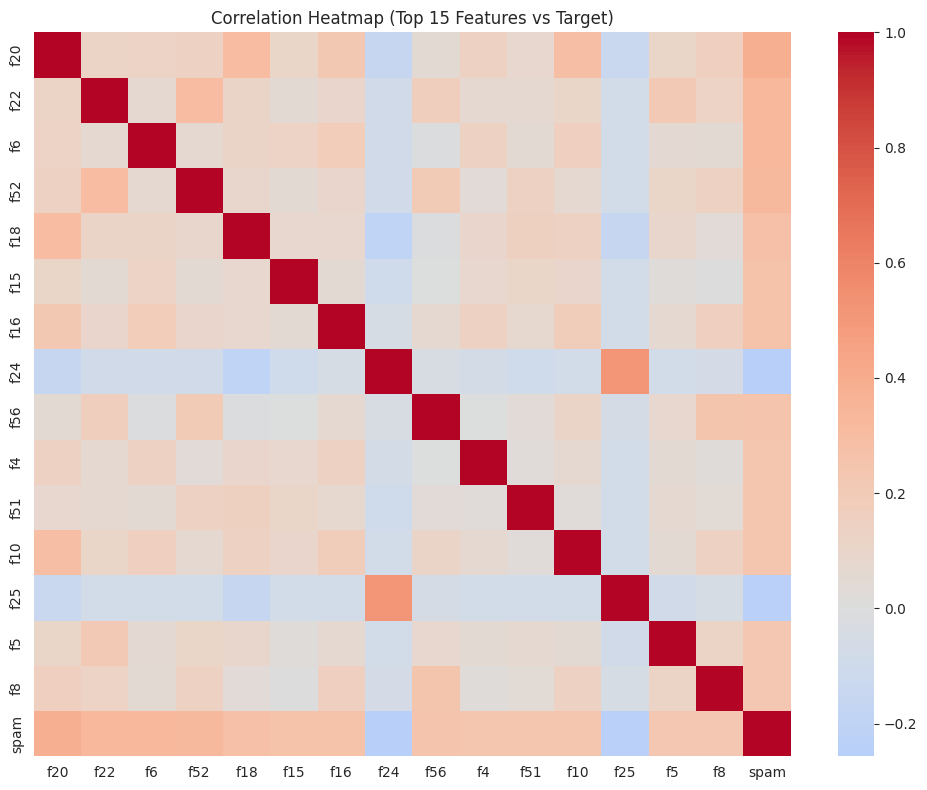
\includegraphics[width=0.85\linewidth]{images/fig02_correlation_heatmap.png}
\caption{Correlation heatmap of the top 15 features most correlated with the spam target.}
\label{fig:corr}
\end{figure}

\textbf{Inference:} The top 15 features selected by absolute correlation with the
target show generally weak-to-moderate positive correlation with \texttt{spam} (mostly
in the 0.1--0.3 range), with feature \texttt{f24} standing out as negatively correlated
with the target and with several other top features. No pair of features shows a very
strong (near 1.0) correlation, suggesting limited redundancy among the top predictive
features and that most of them contribute complementary information.

\begin{figure}[H]
\centering
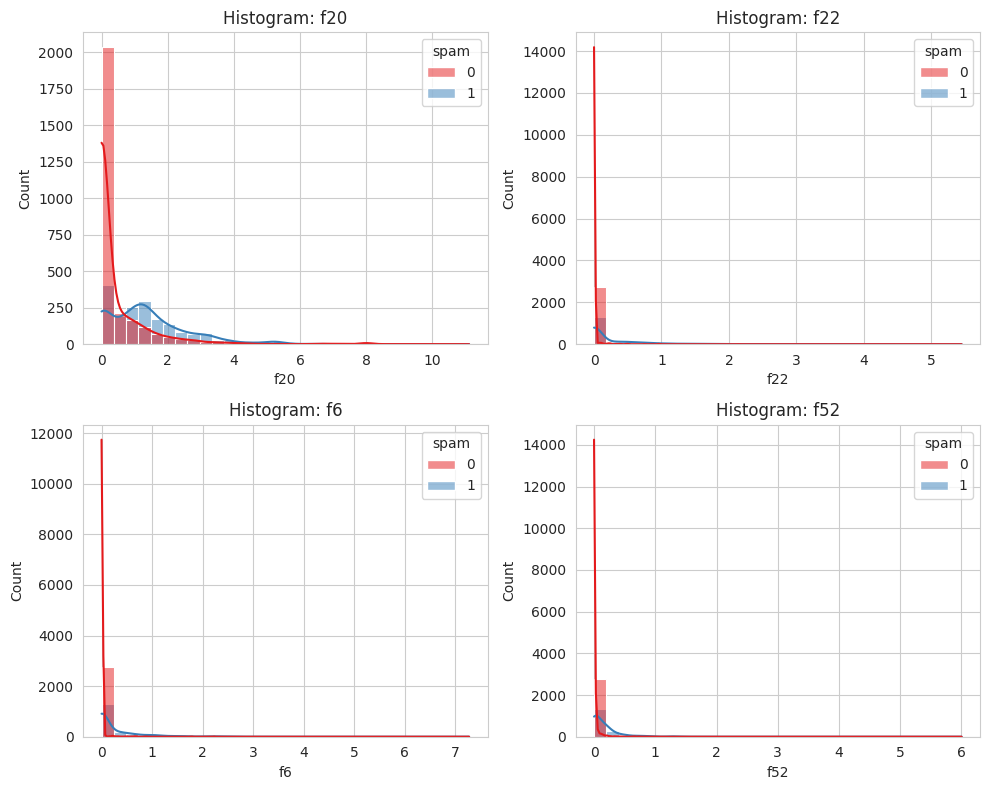
\includegraphics[width=0.85\linewidth]{images/fig03_histograms.png}
\caption{Histograms of the four most target-correlated features, split by class.}
\label{fig:hist}
\end{figure}

\textbf{Inference:} All four features (\texttt{f20}, \texttt{f22}, \texttt{f6},
\texttt{f52}) are heavily right-skewed with most emails having a value near zero.
Spam emails (blue) show a visibly wider spread and higher density at larger feature
values compared to ham emails (red), confirming these features carry useful
discriminative signal. This skew also motivates the use of Multinomial/Bernoulli NB
(suited to frequency/count-style data) and feature scaling for Gaussian NB and KNN.

\begin{figure}[H]
\centering
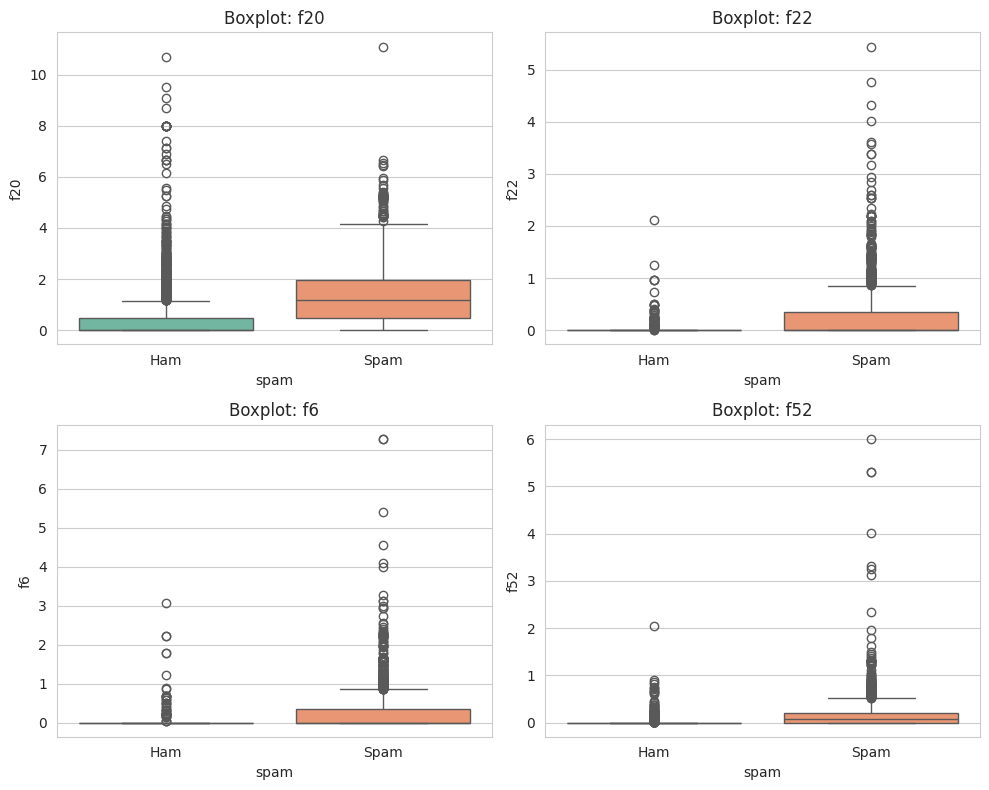
\includegraphics[width=0.85\linewidth]{images/fig04_boxplots.png}
\caption{Boxplots of the four most target-correlated features, grouped by class.}
\label{fig:box}
\end{figure}

\textbf{Inference:} The boxplots confirm that spam emails have a visibly higher median
and interquartile range for all four features compared to ham emails, with numerous
high-value outliers present in both classes. This separation between class medians
supports the predictive value of these features and explains why relatively simple
classifiers such as Na\"ive Bayes and KNN can perform well on this dataset.

\section{Data Preprocessing}
\begin{itemize}
\item \textbf{Missing value handling:} No missing values were present in the dataset;
the pipeline includes a defensive mean-imputation step (\texttt{fillna} with column
mean) that was not triggered here since none were found.
\item \textbf{Encoding:} No categorical encoding was required, as all 57 features are
already numeric (frequency/statistics-based).
\item \textbf{Feature scaling:} Two different scalers were applied depending on model
requirements: \textbf{StandardScaler} (zero mean, unit variance) was used for Gaussian
NB and KNN, which can naturally handle negative/standardized values; \textbf{MinMaxScaler}
(range $[0,1]$) was used for Multinomial NB and Bernoulli NB, which require non-negative
input features.
\item \textbf{Train-test split:} An initial stratified 75/25 train-test split
(\texttt{test\_size=0.25}, \texttt{random\_state=42}) was used for the main
comparisons, preserving the original class ratio in both partitions.
\item \textbf{Feature engineering:} No new derived features were created; all 57
original Spambase attributes were used directly.
\end{itemize}

\section{Machine Learning Algorithms}

\subsection*{Na\"ive Bayes}
\begin{itemize}
\item \textbf{Working principle:} Applies Bayes' theorem with the "naive" assumption
that all features are conditionally independent given the class, and predicts the class
with the highest posterior probability.
\item \textbf{Mathematical formulation:} For a feature vector
$X = (x_1, x_2, \dots, x_n)$,
\begin{equation}
\hat{C} = \arg\max_{C} \; P(C) \prod_{i=1}^{n} P(x_i \mid C)
\end{equation}
Gaussian NB models $P(x_i \mid C)$ as a Gaussian distribution; Multinomial NB models
it as a multinomial (count-based) distribution; Bernoulli NB models it as a Bernoulli
(binary presence/absence) distribution.
\item \textbf{Advantages:} Extremely fast to train ($O(nd)$) and predict ($O(d)$),
performs well even with relatively little training data, and works well for
high-dimensional, frequency-style features (Multinomial/Bernoulli variants).
\item \textbf{Limitations:} The conditional-independence assumption is rarely true in
practice, which can hurt calibration of predicted probabilities; Gaussian NB in
particular can underperform when features are not normally distributed.
\end{itemize}

\subsection*{K-Nearest Neighbors (KNN)}
\begin{itemize}
\item \textbf{Working principle:} A lazy learner that stores the training data and, at
prediction time, finds the $k$ closest training points to a query (by a distance
metric) and assigns the majority class among them.
\item \textbf{Mathematical formulation:} For a query point $x_q$, the predicted class is
\begin{equation}
\hat{C} = \mathrm{mode}\big(\{\, y_i : x_i \in N_k(x_q) \,\}\big)
\end{equation}
where $N_k(x_q)$ is the set of the $k$ nearest training points to $x_q$, typically under
Euclidean distance $d(x_i, x_q) = \sqrt{\sum_j (x_{ij} - x_{qj})^2}$ or Manhattan
distance $d(x_i, x_q) = \sum_j |x_{ij} - x_{qj}|$.
\item \textbf{Advantages:} Simple, non-parametric (makes no assumption about the
underlying data distribution), and can model complex, non-linear decision boundaries.
\item \textbf{Limitations:} Prediction is computationally expensive for large datasets
($O(nd)$ per query in brute-force form), sensitive to feature scaling and irrelevant
features, and requires storing the entire training set in memory.
\end{itemize}

\section{Experimental Setup}
\begin{tabular}{ll}
\toprule
Python Version & 3.x (Jupyter Notebook environment) \\
Scikit-Learn Version & As installed in the notebook environment (\texttt{sklearn}) \\
IDE & Jupyter Notebook \\
Operating System & Notebook host OS (not explicitly logged in the notebook) \\
Hardware & Standard CPU (no GPU-specific code used) \\
\bottomrule
\end{tabular}

\section{Hyperparameter Selection}

\begin{tabular}{ll}
\toprule
Parameter & Value\\
\midrule
KNN $k$ values tested & 1, 3, 5, 7, 9, 11 \\
GridSearchCV \texttt{n\_neighbors} grid & 1, 3, 5, 7, 9, 11, 13, 15 \\
GridSearchCV \texttt{weights} grid & uniform, distance \\
GridSearchCV \texttt{algorithm} grid & auto, ball\_tree, kd\_tree \\
GridSearchCV \texttt{metric} grid & euclidean, manhattan \\
Cross-validation folds (tuning \& evaluation) & 5 (Stratified K-Fold) \\
Train-test split & 75\% / 25\%, stratified, \texttt{random\_state=42} \\
\bottomrule
\end{tabular}

\section{Results}

\subsection*{Na\"ive Bayes Comparison}
\begin{tabular}{lccc}
\toprule
Metric & Gaussian NB & Multinomial NB & Bernoulli NB \\
\midrule
Accuracy  & 0.8254 & 0.9001 & 0.8836 \\
Precision & 0.7077 & 0.9472 & 0.8738 \\
Recall    & 0.9493 & 0.7907 & 0.8238 \\
F1-score  & 0.8109 & 0.8619 & 0.8481 \\
ROC-AUC   & 0.9368 & 0.9614 & 0.9478 \\
\bottomrule
\end{tabular}

\subsection*{KNN Comparison (varying $k$, StandardScaler features)}
\begin{tabular}{ccccc}
\toprule
$k$ & Accuracy & Precision & Recall & F1 \\
\midrule
1  & 0.8975 & 0.8733 & 0.8656 & 0.8695 \\
3  & 0.9018 & 0.8814 & 0.8678 & 0.8746 \\
5  & 0.8992 & 0.8789 & 0.8634 & 0.8711 \\
7  & 0.9053 & 0.8929 & 0.8634 & 0.8779 \\
9  & 0.9062 & 0.8932 & 0.8656 & 0.8792 \\
11 & 0.9027 & 0.8904 & 0.8590 & 0.8744 \\
\bottomrule
\end{tabular}

\textbf{Best $k$: 9} (highest test accuracy of 0.9062 and highest F1 of 0.8792 among
the tested values).

\subsection*{GridSearchCV vs.\ RandomizedSearchCV}
\begin{tabular}{lcc}
\toprule
Parameter & GridSearchCV & RandomizedSearchCV \\
\midrule
Best $k$      & 9         & 15 \\
Metric        & manhattan & manhattan \\
Weights       & distance  & distance \\
Algorithm     & auto      & auto \\
CV Accuracy   & 0.9226    & 0.9200 \\
Execution Time (s) & 50.07 & 7.40 \\
\bottomrule
\end{tabular}

\subsection*{KDTree vs.\ BallTree}
\begin{tabular}{lcc}
\toprule
Metric & KDTree & BallTree \\
\midrule
Accuracy         & 0.9062  & 0.9062 \\
Training Time (s) & 0.0117 & 0.0086 \\
Prediction Time (s) & 0.2412 & 0.2292 \\
\bottomrule
\end{tabular}

\subsection*{5-Fold Cross Validation}
\begin{tabular}{lcc}
\toprule
Fold & Na\"ive Bayes (Multinomial NB) & Best KNN \\
\midrule
1 & 0.8855 & 0.9130 \\
2 & 0.8971 & 0.9290 \\
3 & 0.8942 & 0.9377 \\
4 & 0.8826 & 0.9232 \\
5 & 0.8812 & 0.9130 \\
\midrule
\textbf{Average} & \textbf{0.8881} & \textbf{0.9232} \\
\bottomrule
\end{tabular}

\subsection*{Theoretical Time Complexity}
\begin{tabular}{lcc}
\toprule
Algorithm & Training & Prediction \\
\midrule
Na\"ive Bayes & $O(nd)$ & $O(d)$ \\
KNN (Brute) & $O(1)$ & $O(nd)$ \\
KDTree & $O(n\log n)$ & $O(\log n)_{avg}$ \\
BallTree & $O(n\log n)$ & $O(\log n)_{avg}$ \\
\bottomrule
\end{tabular}

\subsection*{Experimental Time Analysis}
\begin{tabular}{lcc}
\toprule
Algorithm & Training(s) & Prediction(s) \\
\midrule
Gaussian NB & 0.003457 & 0.001520 \\
Multinomial NB & 0.001931 & 0.000280 \\
Bernoulli NB & 0.003831 & 0.000969 \\
Best KNN ($k=9$) & 0.011707 & 0.241179 \\
\bottomrule
\end{tabular}

\section{Result Visualization}

\begin{figure}[H]
\centering
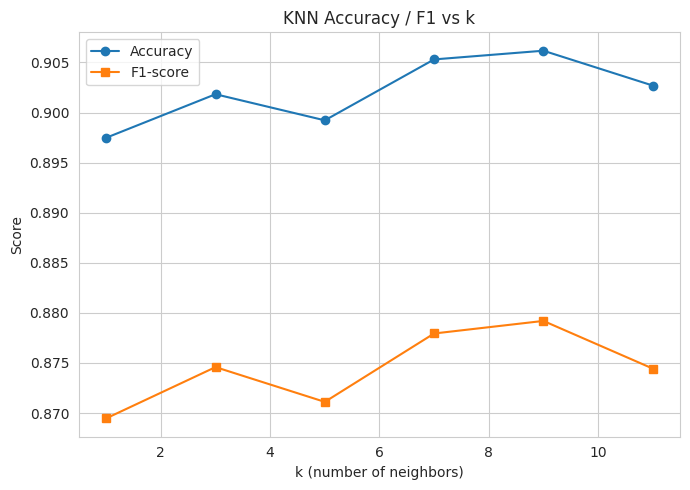
\includegraphics[width=0.75\linewidth]{images/fig05_accuracy_vs_k.png}
\caption{KNN test Accuracy and F1-score as a function of $k$.}
\label{fig:acck}
\end{figure}

\textbf{Inference:} Accuracy and F1-score both rise from $k=1$ to a local peak around
$k=3$, dip slightly at $k=5$, then climb to their maximum near $k=9$ before declining
at $k=11$. This non-monotonic pattern illustrates the classic bias-variance trade-off in
KNN: very small $k$ (e.g., $k=1$) overfits to noise in individual neighbors, while
larger $k$ smooths the decision boundary but can eventually underfit by including
less-relevant neighbors. $k=9$ offers the best balance for this dataset.

\begin{figure}[H]
\centering
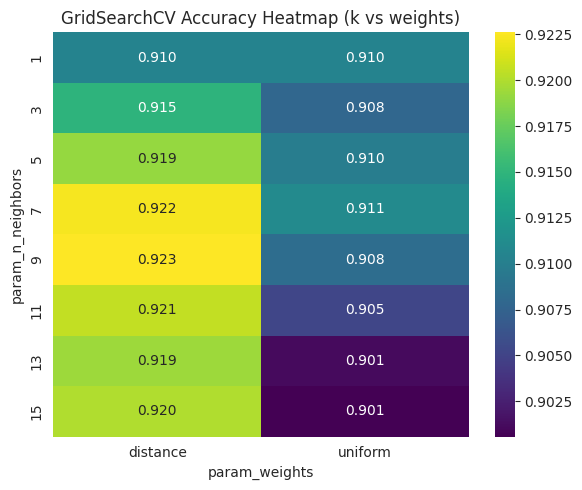
\includegraphics[width=0.75\linewidth]{images/fig06_gridsearch_heatmap.png}
\caption{GridSearchCV mean cross-validation accuracy heatmap ($k$ vs.\ weights, for the best metric = manhattan).}
\label{fig:gridheat}
\end{figure}

\textbf{Inference:} The heatmap shows that the \texttt{distance}-weighted KNN
consistently outperforms \texttt{uniform} weighting across nearly all values of $k$,
with the best combination at $k=9$, \texttt{weights=distance} (CV accuracy $\approx0.923$).
Accuracy generally increases with $k$ up to around 9, then slowly declines, again
reflecting the bias-variance trade-off observed in Figure~\ref{fig:acck}.

\begin{figure}[H]
\centering
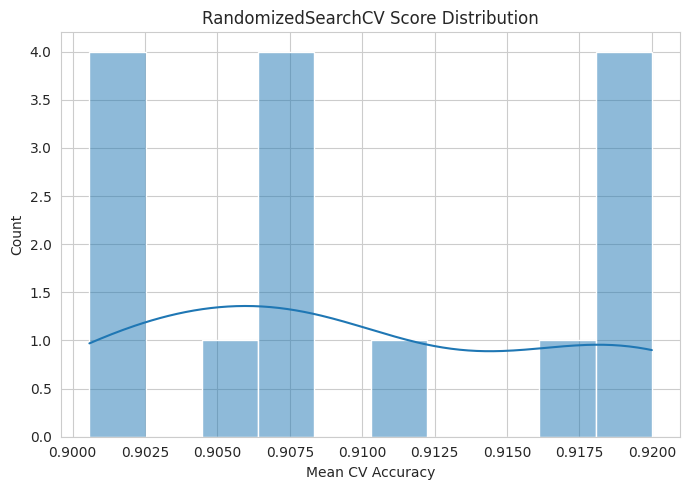
\includegraphics[width=0.75\linewidth]{images/fig07_randomsearch_distribution.png}
\caption{Distribution of mean cross-validation accuracy scores sampled by RandomizedSearchCV.}
\label{fig:randdist}
\end{figure}

\textbf{Inference:} The sampled configurations from RandomizedSearchCV cluster tightly
between approximately 0.900 and 0.920 mean CV accuracy, showing that KNN performance is
fairly stable across a wide range of hyperparameter combinations on this dataset. This
also explains why RandomizedSearchCV, despite sampling only a subset of the full grid,
was able to find a near-optimal configuration (0.9200 vs.\ GridSearchCV's 0.9226) in a
fraction of the time.

\begin{figure}[H]
\centering
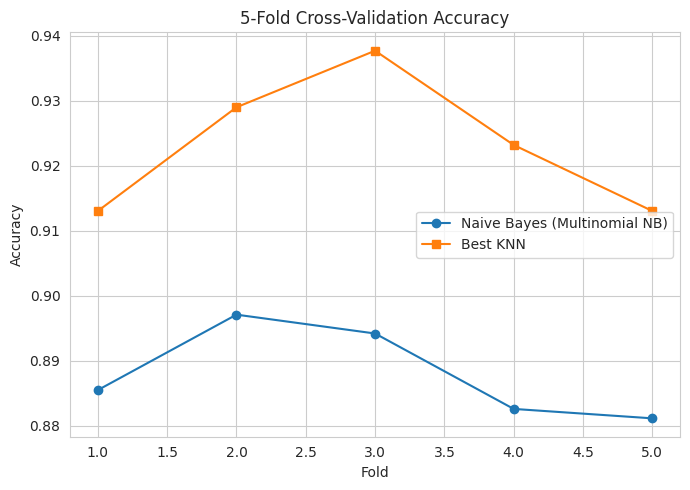
\includegraphics[width=0.75\linewidth]{images/fig08_cv_accuracy.png}
\caption{5-fold cross-validation accuracy per fold for the best Na\"ive Bayes model (Multinomial NB) and the best KNN model.}
\label{fig:cvacc}
\end{figure}

\textbf{Inference:} The best KNN model consistently outperforms Multinomial NB across
all 5 folds, with both models showing some fold-to-fold variability (KNN ranging from
0.913 to 0.938; Multinomial NB ranging from 0.881 to 0.897). The consistent gap between
the two curves indicates that KNN's advantage over Naive Bayes on this dataset is
stable and not an artifact of a single lucky train-test split.

\begin{figure}[H]
\centering
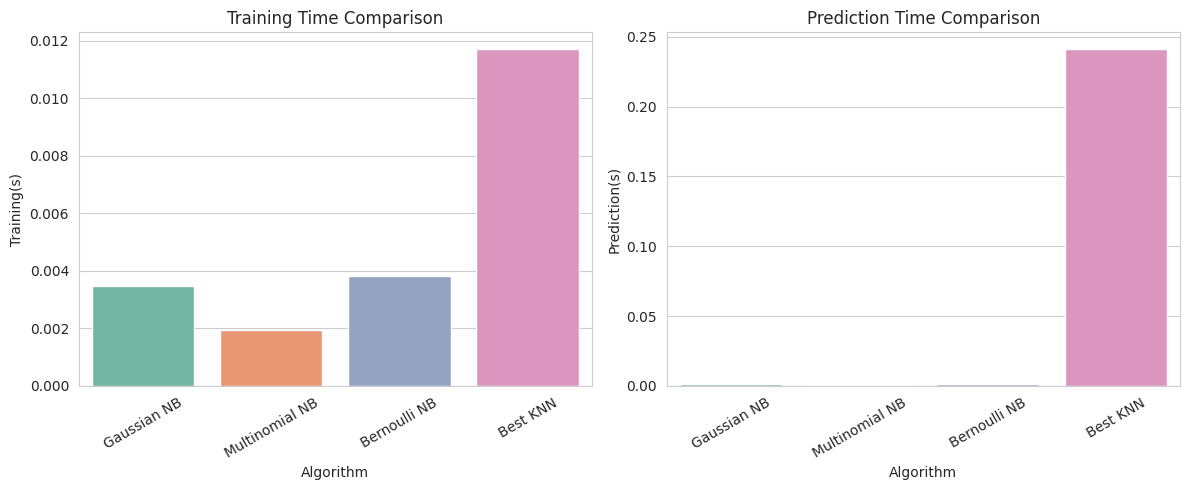
\includegraphics[width=0.9\linewidth]{images/fig09_training_prediction_time.png}
\caption{Training time and prediction time comparison across all four models.}
\label{fig:time}
\end{figure}

\textbf{Inference:} All three Na\"ive Bayes variants train and predict in a few
milliseconds, while KNN's training time is also small (since it only stores/indexes
the data) but its prediction time is dramatically higher (over 0.24s on the test set),
roughly 100$\times$ slower than any Na\"ive Bayes variant. This empirically confirms the
theoretical expectation that KNN shifts computational cost from training to prediction.

\begin{figure}[H]
\centering
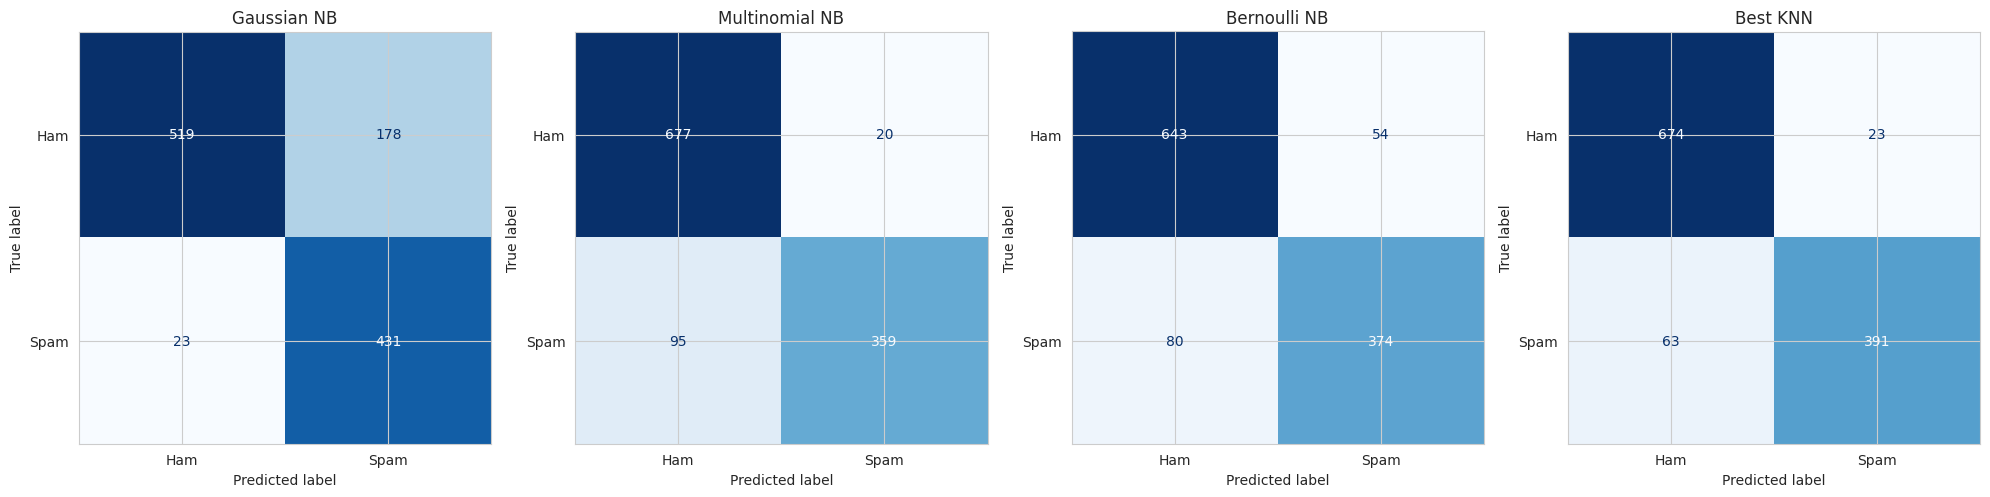
\includegraphics[width=0.95\linewidth]{images/fig10_confusion_matrices.png}
\caption{Confusion matrices for Gaussian NB, Multinomial NB, Bernoulli NB, and Best KNN.}
\label{fig:cm}
\end{figure}

\textbf{Inference:} Gaussian NB shows the most false positives (178 ham emails
misclassified as spam), consistent with its lower precision. Multinomial NB has very
few false positives (20) but more false negatives (95), reflecting its high precision
but lower recall. Best KNN achieves the best overall balance, with only 23 false
positives and 63 false negatives, consistent with it having the highest accuracy and
F1-score among all four models.

\begin{figure}[H]
\centering
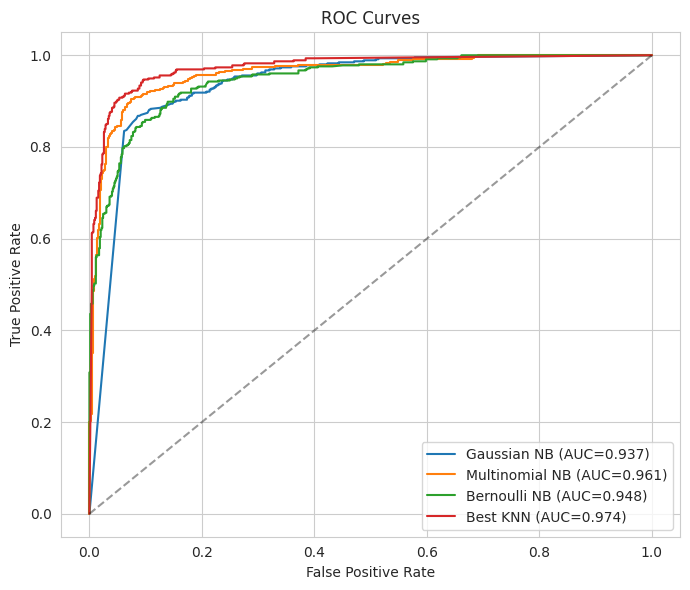
\includegraphics[width=0.7\linewidth]{images/fig11_roc_curves.png}
\caption{ROC curves for all four classifiers.}
\label{fig:roc}
\end{figure}

\textbf{Inference:} Best KNN achieves the highest AUC (0.974), followed by Multinomial
NB (0.961), Bernoulli NB (0.948), and Gaussian NB (0.937). All four curves rise steeply
toward the top-left corner, indicating strong overall discriminative ability, but KNN's
curve dominates the others across almost the entire false-positive-rate range,
confirming it is the strongest classifier by ranking quality as well as by raw accuracy.

\begin{figure}[H]
\centering
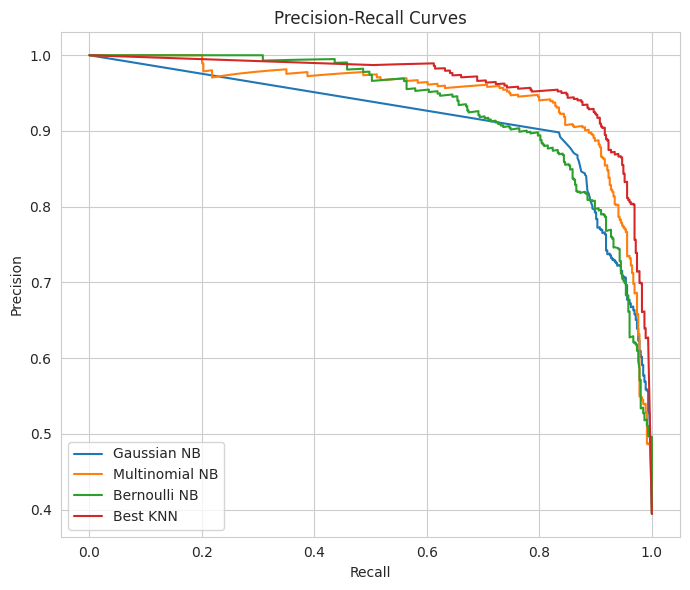
\includegraphics[width=0.7\linewidth]{images/fig12_pr_curves.png}
\caption{Precision-Recall curves for all four classifiers.}
\label{fig:pr}
\end{figure}

\textbf{Inference:} Bernoulli NB and Multinomial NB maintain very high precision at low
recall, but their precision drops off faster than Best KNN's as recall increases.
Gaussian NB has the weakest precision-recall trade-off throughout, consistent with its
lower F1-score. Best KNN maintains the best precision across most of the recall range,
reinforcing its position as the top-performing model on this imbalanced dataset.

\begin{figure}[H]
\centering
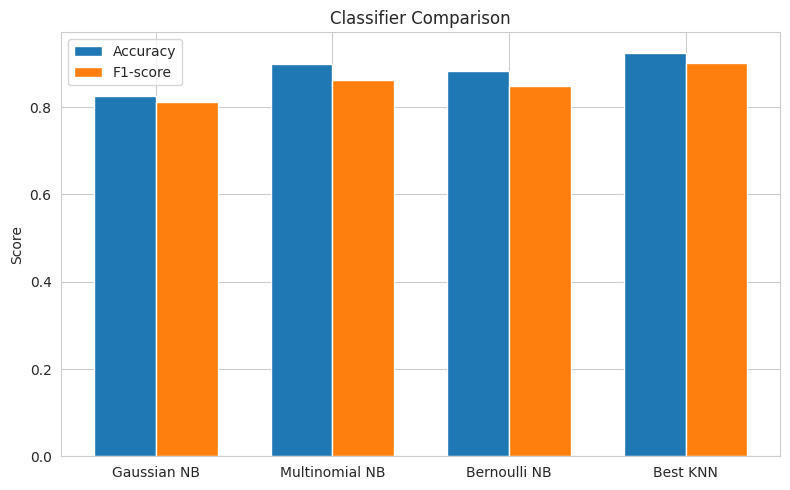
\includegraphics[width=0.75\linewidth]{images/fig13_classifier_comparison.png}
\caption{Overall Accuracy and F1-score comparison across all four classifiers.}
\label{fig:compare}
\end{figure}

\textbf{Inference:} Best KNN achieves the highest Accuracy ($\approx0.926$) and F1-score
($\approx0.90$) among all four models, followed by Multinomial NB. Gaussian NB is the
weakest performer on both metrics. This summary chart consolidates the individual
metric tables (Section~7) into a single visual comparison, making the overall ranking
of classifiers immediately clear: \textbf{Best KNN $>$ Multinomial NB $>$ Bernoulli NB
$>$ Gaussian NB}.

\section{Additional Tasks}

\subsection*{Different Train-Test Splits}
\begin{tabular}{cc}
\toprule
Test Size & Accuracy \\
\midrule
0.20 & 0.9088 \\
0.25 & 0.9062 \\
0.30 & 0.9073 \\
0.40 & 0.9028 \\
\bottomrule
\end{tabular}

KNN accuracy is fairly stable (within about 0.6 percentage points) across test sizes
ranging from 20\% to 40\%, with the smallest test size (20\%, more training data)
giving the best accuracy and the largest test size (40\%, less training data) giving
the lowest, as expected.

\subsection*{Euclidean vs.\ Manhattan Distance}
\begin{tabular}{lc}
\toprule
Metric & Accuracy \\
\midrule
Euclidean & 0.9062 \\
Manhattan & 0.9131 \\
\bottomrule
\end{tabular}

Manhattan distance outperforms Euclidean distance by about 0.7 percentage points at
$k=9$ on this dataset, which is also reflected in GridSearchCV independently selecting
\texttt{manhattan} as the best metric.

\subsection*{Weighted KNN (Uniform vs.\ Distance)}
\begin{tabular}{lc}
\toprule
Weights & Accuracy \\
\midrule
Uniform & 0.9062 \\
Distance & 0.9140 \\
\bottomrule
\end{tabular}

Distance-weighted voting improves accuracy by about 0.8 percentage points over uniform
voting at $k=9$, since it gives closer neighbors more influence over the predicted
class, reducing the impact of farther, potentially less-relevant neighbors.

\subsection*{Overfitting vs.\ Underfitting in KNN}
Small values of $k$ (e.g., $k=1$) make the model highly sensitive to individual noisy
training points, leading to a jagged, overly complex decision boundary that
\textbf{overfits} the training data -- this is reflected in Figure~\ref{fig:acck}, where
$k=1$ has the lowest accuracy and F1 among the small-$k$ values tested. Conversely,
very large values of $k$ smooth the decision boundary excessively, causing the model to
\textbf{underfit} by ignoring local structure in the data and relying on an
increasingly global, less discriminative vote; this begins to show as the mild
performance drop from $k=9$ to $k=11$ in the same figure.

\section{Discussion}
Among the three Na\"ive Bayes variants, \textbf{Multinomial NB} achieved the highest
accuracy (0.900), precision (0.947), F1-score (0.862), and ROC-AUC (0.961), which
aligns with theoretical expectations since the Spambase features are frequency/count
statistics rather than normally distributed continuous values -- the assumption
underlying Gaussian NB. Gaussian NB had the highest recall (0.949) but at a steep cost
in precision (0.708), meaning it flags many ham emails as spam.

For KNN, accuracy improved as $k$ increased from 1 up to 9, then declined slightly at
$k=11$, and hyperparameter tuning via GridSearchCV confirmed $k=9$ with Manhattan
distance and distance-based weighting as the best configuration (CV accuracy 0.923).
RandomizedSearchCV found a comparable configuration (CV accuracy 0.920, with $k=15$)
in roughly $1/7$ of GridSearchCV's execution time (7.4s vs.\ 50.1s), demonstrating a
practical, favorable trade-off between search thoroughness and computational cost when
the hyperparameter search space is small enough that a randomized subset still
captures near-optimal regions. KDTree and BallTree produced identical accuracy (as
expected, since both compute exact nearest neighbors), differing only in construction
and query time, with BallTree being marginally faster on this particular run.

Comparing theoretical and empirical complexity: Na\"ive Bayes' training and prediction
times were consistently in the low milliseconds, matching its $O(nd)$/$O(d)$
theoretical bounds. KNN's training time was also small (index construction only), but
its prediction time was roughly $100\times$ larger than any Na\"ive Bayes variant,
empirically confirming the $O(nd)$ per-query prediction cost of brute-force /
tree-based KNN search on this dataset size. This makes \textbf{Na\"ive Bayes strongly
preferable for large-scale or latency-sensitive deployments}, while KNN remains
attractive when maximum predictive accuracy is the priority and the dataset/query
volume is manageable.

A limitation of this study is that the dataset was loaded using generic column names
(\texttt{f0}--\texttt{f56}) rather than the semantic Spambase attribute names (e.g.,
\texttt{word\_freq\_free}, \texttt{char\_freq\_!}), since the Kaggle CSV with headers
was not available in the working directory and the pipeline fell back to the
header-less UCI \texttt{.data} file. This does not affect any numerical result but
limits direct semantic interpretation of which specific words/characters are most
predictive of spam.

\section{Conclusion}
This experiment successfully implemented and compared Na\"ive Bayes (Gaussian,
Multinomial, Bernoulli) and KNN classifiers on the UCI Spambase dataset (4601 emails,
57 features). \textbf{Multinomial NB} was the best-performing Na\"ive Bayes variant, and
\textbf{KNN with $k=9$, Manhattan distance, and distance-weighting} (selected via
GridSearchCV) was the overall best-performing model, achieving the highest accuracy
(0.926 on 5-fold CV average) and ROC-AUC (0.974) among all four classifiers, at the
cost of substantially higher prediction time than any Na\"ive Bayes variant.
GridSearchCV and RandomizedSearchCV converged on similar optimal regions of the
hyperparameter space, with RandomizedSearchCV offering a much faster alternative for
larger search spaces. KDTree and BallTree produced identical accuracy with comparable
speed. Overall, the experiment reinforced key theoretical concepts -- the
bias-variance trade-off in $k$, the importance of matching a Na\"ive Bayes variant's
distributional assumption to the data, and the practical training/prediction time
trade-off between eager (Na\"ive Bayes) and lazy (KNN) learners.

\section{References}
\begin{enumerate}
\item F. Pedregosa \textit{et al.}, "Scikit-learn: Machine Learning in Python," \textit{Journal of Machine Learning Research}, vol. 12, pp. 2825--2830, 2011.
\item A. G\'eron, \textit{Hands-On Machine Learning with Scikit-Learn, Keras and TensorFlow}, 2nd ed. O'Reilly Media, 2019.
\item C. M. Bishop, \textit{Pattern Recognition and Machine Learning}. Springer, 2006.
\item M. Hopkins, E. Reeber, G. Forman, and J. Suermondt, "Spambase," UCI Machine Learning Repository, 1999. [Online]. Available: \url{https://doi.org/10.24432/C53G6X}
\item Kaggle Datasets, "Spambase Dataset," \url{https://www.kaggle.com/datasets/somesh24/spambase}, accessed 2026.
\end{enumerate}

\end{document}
